\chapter{Time Series Analysis: 
ARMA and VAR}\label{ch-time-arma}



This chapter is based mostly 
on the book  Ref.\cite{hamilton2020time}
on time series analysis by Hamilton, 
and on the lectures Ref. \cite{t-series-kuan}
by Chung-Ming Kuan.
In writing this chapter, we also profited greatly
from numerous Wikipedia entries on time series
analysis,
such as  the entries
on 
time series (Ref.\cite{wiki-time-series}),
ARMA time series (Ref.\cite{wiki-ARMA}),
AR time series (Ref.\cite{wiki-AR}),
MA time series (Ref.\cite{wiki-MA}), and
VAR time series (Ref.\cite{wiki-VAR}).



We cover only a small fraction
 of the  treasures
covered in those sources, 
and only
cover stationary 
time-series. Non-stationary 
time series
we don't even touch.
But we hope to have covered 
enough to pique 
our readers's interest in time series analysis,
and make him/her appreciate
how bnets make
 time series much more 
intuitive and fun.
The time-series 
considered in this chapter
can 
be represented 
by one of the
simplest
types of
bnets, namely, the LDEN bnets
introduced in 
Chapter \ref{ch-linear-sys}.



As usual, for $t, t_a, t_b\in \ZZ$,
 let
 $\ZZ_{<t}=
\{t-1, t-2, t-3, \ldots\}$,
$\ZZ_{[t_a, t_b]}=\{t_a, t_a+1, 
\ldots, t_b\}$, etc.

Let $\rvx_t\in \RR$.
A 
{\bf time series (t-series)},
denoted variously by
$\{\rvx_1, \rvx_2, \ldots,
\rvx_{nt}\}
=\{\rvx_t\}_{t=1}^{nt}
=\tseries{\rvx_t}$,
is a set of real numbers
index by a discrete set of times
$\ZZ_{[0, nt]}$.


For $t_a<t_b$, let 
$\rvx_{[t_a, t_b]}=(\rvx_{t_a}, 
\rvx_{t_a+1},
 \ldots, \rvx_{t_b})$.
Let $x_{<t}=(\ldots, x_{t-2}, \rvx_{t-1})$.

\section{White noise}

By {\bf white noise} 
$\tseries{\rvn_t}\sim  WN(0, \s^2)$
we mean a t-series $\tseries{\rvn_t}$
that satisfies

\beq
E[\rvn_t]=0
\eeq
and

\beq
\av{\rvn_t,\rvn_{t'}}=\s^2\delta(t,t')
\;.
\eeq
{\bf Gaussian white noise}
$\tseries{\rvn_t}\sim WN(0, \s^2)_\caln$
is white noise such that also
$\rvn_t\sim \caln(0, \s^2)$.

\section{Backshift operator}

$\calb$ is the backshift (a.k.a. lag) operator.
For any t-series $\tseries{x_t}$,
$\tseries{y_t}$
and scalars $a, b\in \RR$, 

\beq
\calb \rvx_t=\rvx_{t-1}
\eeq

\beq
\calb(a\rvx_t + b \rvy_t)=
a\calb(\rvx_t) + b\calb(\rvy_t)
\eeq
A $\calb$ Polynomial
with coefficients $\alp_{[0,p]}$:
\beq
\alp(\calb)= \alp_0 + \alp_1\calb 
+ \alp_2\calb^2 +\ldots \alp_p\calb^p
\eeq
$\calb^{-1}$ is the inverse of 
the backshift operator
 (a.k.a. frontshift operator) 
\beq
\calb^{-1}\rvx_t=\rvx_{t+1}
\eeq

The following two 
Taylor expansions
prove useful 
in finding the inverse
of backshift operator 
polynomials:
\begin{itemize}
\item
\beq
\frac{1}{1-z}=1+z+z^2+\ldots
\label{eq-binomial-expan}
\eeq
converges for $z\in \CC$ with $|z|<1$.
 We will use this expansion with $z$ replaced
by $\alp \calb$, where $\alp\in\RR$.

\item

\beq
\frac{1}{1-z}=
(-z^{-1})
\left[\frac{1}{1-z^{-1}}\right]
=
(-z^{-1})
\left[
1 + z^{-1} + 
+ z^{-2} + \ldots
\right]
\label{eq-binomial-expan-inv-z}
\eeq
converges for $z\in \CC$ 
with $|z|>1$. We will use this expansion 
with $z^{-1}$ replaced
by $(\alp \calb)^{-1}$, where $\alp\in\RR$.
\end{itemize}

\section{Metrics}

Consider a t-series $\tseries{\rvx_t}$.

In general, if we have a metric 
like Auto-covariance (ACov) that
is defined for $\tau=1,2,3, \ldots$,
it is 
conventional in time series analysis to refer to
the plot of that metric
for all values of $\tau$ 
as the Auto-covariance {\it Function} (ACovF).

\begin{itemize}

\item {\bf Expected value and Variance}

\beq
E[\rvx_t]
\eeq

\beq
Var[\rvx_t]=\av{\rvx_t, \rvx_t}
\eeq

\item{\bf Auto-covariance (ACov)}

\beq
\gamma_{t, t+\tau}
=\av{\rvx_t, \rvx_{t+\tau}}
\eeq




\item{\bf Auto-correlation (ACorr)} (assumes
w-stationarity)

\beq
\rho(\tau)=
\frac{\gamma(\tau)}{\gamma(0)}
\eeq

\item {\bf Generating function 
of auto-covariance} (assumes w-stationarity)


\beq
\tilde{\gamma}(z)=\sum_{\tau=-\infty}^{\infty}
\gamma(\tau) z^\tau
\eeq
Note that this transform is double sided.
Fourier Transform 
if $z=e^{-i\omega\tau}$.

\item{\bf Expected value 
and variance conditioned on all past information}

For $\tau=1,2, 3, \dots$,

\beq
E_{|x_{\leq t}}[\rvx_{t+\tau}]
\eeq

\beq
Var_{|x_{\leq t}}[\rvx_{t+\tau}]
=
\av{\rvx_{t+\tau},
\rvx_{t+\tau}}_{|x_{\leq t}}
\eeq

\item {\bf Partial auto-covariance (PACov)}

Assume w-stationarity.
For $\tau=1,2,3, \ldots$
\beq
\gamma^{part}(\tau)=
\av{\rvx_t, \rvx_{t+\tau}}_{|x_{\leq t}, \rvx_{t+\tau}}
\eeq
The idea is that we set to zero the
nodes $\rvx_{(t, t+\tau)}=
\{\rvx_{t+1}, \rvx_{t+2}, \ldots,\rvx_{t+\tau-1}\}$ 
that lie
between 
(but not including) $\rvx_t$ and $\rvx_{t+\tau}$.

\item {\bf Partial auto-correlation (PACorr)}


\beq
\rho^{part}(\tau)=
\frac{\gamma^{part}(\tau)}
{\gamma^{part}(0)}
\eeq
\end{itemize}


\hrule

{\bf weak stationarity (w-stationarity)}
means that
$E[\rvx_t]=\mu$ 
and 
$\gamma_{t, t+\tau}=\gamma(\tau)$
are both independent of $t$.
If we have w-stationarity, 
then

\beqa
\gamma(-\tau)&=&
\av{\rvx_t, \rvx_{t-\tau}}
\\
&=&
\av{\rvx_{t-\tau}, \rvx_t}
\\
&=&
\gamma (\tau)
\eeqa

We will often abbreviate $\gamma(\tau)$ by $\gamma_\tau$.

Example of various metrics.
If $\tseries{\rvn_t}
\sim WN(0, \s^2)$ then

\begin{subequations}
\beq
E[\rvn_t]=0
\eeq

\beq
\gamma(\tau)=\s^2
\delta(\tau,0)
\eeq


\beq
\gamma(0)=\s^2
\eeq



\beq
\tilde{\gamma}(z)=\gamma(0)
\eeq

For $\tau>0$, 
\beq
E_{|n_{\leq t}}[\rvn_{t+\tau}]=
E[\rvn_{t+\tau}]=0
\eeq

\beq
\av{\rvn_{t+\tau}, \rvn_{t+\tau}}_{|n_{\leq t}}=
E[\rvn_{t+\tau}^2]=
\s^2
\eeq
\end{subequations}


\section{
Definition of $ARMA(p,q)$,
$AR(p)$ and $MA(q)$.}

\begin{figure}[h!]
$$
\begin{array}{c}
ARMA(2,3)\\
\xymatrix@C=36px{
\cdots
\rvn_{t-4}
&\rvn_{t-3}\ar[drrr]^{\nu_3}
&\rvn_{t-2}\ar[drr]^{\nu_2}
&\rvn_{t-1}\ar[dr]^{\nu_1}
&\rvn_t\ar[d]^1
&\rvn_{t+1}
&\rvn_{t+2}
\cdots
\\
\cdots
\rvy_{t-4}
&\rvy_{t-3}
&\rvy_{t-2}\ar@/_1pc/[rr]_{\alp_2}
&\rvy_{t-1}\ar[r]_{\alp_1}
&{\color{red}\rvy_t}
&\rvy_{t+1}&\rvy_{t+2}
\cdots
}
\\
\\
AR(2)\\
\xymatrix@C=36px{
\cdots
\rvn_{t-4}
&\rvn_{t-3}
&\rvn_{t-2}
&\rvn_{t-1}
&\rvn_t\ar[d]^1
&\rvn_{t+1}
&\rvn_{t+2}
\cdots
\\
\cdots
\rvy_{t-4}
&\rvy_{t-3}
&\rvy_{t-2}\ar@/_1pc/[rr]_{\alp_2}
&\rvy_{t-1}\ar[r]_{\alp_1}
&{\color{red}\rvy_t}
&\rvy_{t+1}&\rvy_{t+2}
\cdots
}
\\
\\
MA(3)\\
\xymatrix@C=36px{
\cdots
\rvn_{t-4}
&\rvn_{t-3}\ar[drrr]^{\nu_3}
&\rvn_{t-2}\ar[drr]^{\nu_2}
&\rvn_{t-1}\ar[dr]^{\nu_1}
&\rvn_t\ar[d]^1
&\rvn_{t+1}
&\rvn_{t+2}
\cdots
\\
\cdots
\rvy_{t-4}
&\rvy_{t-3}
&\rvy_{t-2}
&\rvy_{t-1}
&{\color{red}\rvy_t}
&\rvy_{t+1}&\rvy_{t+2}
\cdots
}
\end{array}
$$
\caption{$ARMA(2,3)$,
$AR(2)$ and $MA(3)$ bnets.
 For clarity, we show  only the
 arrows entering node $\rvy_t$.
The full bnet has the same
structural  pattern of incoming arrows
(including the  weights $\alp_j, \nu_j$)
for each node  $\rvy_{t'}$ 
for all $t'$.
}
\label{fig-single-node-arma-2-3}
\end{figure}

Suppose $\tseries{\rvy_t}$
is a zero mean t-series. Hence
$\rvy_t= \rvY_t-\mu$, 
$E[\rvY_t]=\mu$,
$E[\rvy_t]=0$. 
$\rvy_t$ is said to be the {\bf demeaned}
version of $Y_t$.

Suppose also that
$\tseries{\rvn_t}\sim WN(0, \s^2)$. 

Then we define the
{\bf Auto-Regressive Moving-Average 
t-series} $ARMA(p,q)$ by

\beq
\rvy_t=
\underbrace{\sum_{j=1}^p\alp_j \rvy_{t-j}}_
{\caly^{AR(p)}_t}
+ \rvn_t +
\underbrace{\sum_{j=1}^q
\nu_j \rvn_{t-j}
}_{\caly^{MA(q)}_t}
\label{eq-arma-def}
\eeq($\alp$ stands for 
the first  letter
of ``auto-regressive".
$\nu$ stands for first
 letter of ``noise".)


Special cases
\begin{enumerate}
\item  {\bf Auto-Regressive t-series} $AR(p)$

\beq
\rvy_t =
\caly^{AR(p)}_t
+ \rvn_t
\label{eq-ar-def}
\eeq

\item {\bf Moving-Average t-series}
 $MA(q)$ 

\beq
\rvy_t = \rvn_t  +
\caly^{MA(q)}_t
\label{eq-ma-def}
\eeq
\end{enumerate}




 Fig.\ref{fig-single-node-arma-2-3}
shows the bnets for 
$ARMA(2,3)$, $AR(2)$ and $MA(3)$.
The TPM, printed in blue,
for node $\rvy_t$
in those bnets,
is as follows:

For $ARMA(p,q)$, 
\beq\color{blue}
P(y_t|y_{[t-p   , t-1]}, 
n_{[t-q, t]})
=
\indi(y_t = \text{see Eq.\ref{eq-arma-def}}))
\eeq

For $AR(p)$, 
\beq\color{blue}
P(y_t|y_{[t-p   , t-1]}, 
n_{t})
=
\indi(y_t = \text{see Eq.\ref{eq-ar-def}}))
\eeq

For $MA(q)$,
\beq\color{blue}
P(y_t| 
n_{[t-q, t]})
=
\indi(y_t = \text{see Eq.\ref{eq-ma-def}}))
\eeq



The $\rvn_t$ variable
is variously referred to as the
{\bf external noise, impulse,
shock, innovation}
at time $t$.

\section{Solving $AR(p)$}

Suppose $\tseries{\rvy_t}$ is an $AR(p)$
t-series. Hence

\beq
\rvy_t=\sum_{j=1}^p\alp_jy_{t-j} + \rvn_t
\eeq


$AR(0)$ satisfies:

\beq
\rvy_t=\rvn_t
\eeq
See Fig.\ref{fig-AR-0-1}.
This is just white noise.


$AR(1)$ satisfies:

\beq
\rvy_t= \alp_1 \rvy_{t-1} + \rvn_t
\eeq
See Fig\ref{fig-AR-0-1}.
This  is a Markov chain 
with external i.i.d. noise injected
to each node.
$AR(1)$
is the discrete
form of the
so called {\bf Ornstein-Uhlenbeck
 t-series} (aka as the {\bf Langevin
 Equation}).
 When $\alp_1=1$,
it is called a {\bf random walk}.

\begin{figure}[h!]
$$
\begin{array}{cc}
AR(0)&
\xymatrix{
\cdots
\rvn_{t-2}\ar[d]_1
&\rvn_{t-1}\ar[d]_1
&\rvn_{t}\ar[d]_1
&\rvn_{t+1}\ar[d]_1
\cdots
\\
\cdots
\rvy_{t-2}
&\rvy_{t-1}
&\rvy_{t}
&\rvy_{t+1}
\cdots
}
\\
\\
AR(1)&
\xymatrix{
\cdots
\rvn_{t-2}\ar[d]_1
&\rvn_{t-1}\ar[d]_1
&\rvn_{t}\ar[d]_1
&\rvn_{t+1}\ar[d]_1
\cdots
\\
\cdots
\rvy_{t-2}\ar[r]_{\alp_1}
&\rvy_{t-1}\ar[r]_{\alp_1}
&\rvy_{t}\ar[r]_{\alp_1}
&\rvy_{t+1}
\cdots
}
\end{array}
$$
\caption{Bnets for $AR(0)$ and $AR(1)$.}
\label{fig-AR-0-1}
\end{figure}


Note that

\beq
\alp^-(\calb)
\rvy_t = \rvn_t
\label{eq-ar-alp-minus}
\;
\eeq
where

\beq
\alp^-(\calb)=
1-\sum_{j=1}^p
 \alp_j \calb^j
\eeq
Note that we can get $AR(p)$
from $AR(\infty)$
by setting $\alp_{>p}=0$.


If $\alp^-(\beta)$
is invertible, then, using
the Taylor expansion 
Eq.(\ref{eq-binomial-expan}), we get

\beq
\rvy_t = \alp'(\calb)\rvn_t
\eeq
where

\beq
\alp'(\calb)=
\frac{1}
{\alp^-(\calb)}
=1+\sum_{k=1}^\infty\left[\sum_{j=1}^p\alp_j \calb^j
\right]^k
=\sum_{j=0}^\infty \alp'_j \calb^j
\eeq
where $\alp'_0=1$.








\section{Solving $MA(q)$}

Suppose $\tseries{\rvy_t}$ is an $MA(q)$
t-series. Hence,





\beq
\rvy_t = \rvn_t+
\sum_{j=1}^q
 \nu_j \rvn_{t-j}
=
\sum_{j=0}^q
 \nu_j \rvn_{t-j}
\eeq
where $\nu_0=1$. Thus,


\beq
\rvy_t = 
\nu(\calb)\rvn_t
\label{eq-ma-nu}
\eeq
where

\beq
\nu(\calb)=1+\sum_{j=1}^q \nu_j \calb^j=
\sum_{j=0}^q \nu_j \calb^j
\;.
\eeq
Note that we can get $MA(q)$
from $MA(\infty)$
by setting $\nu_{>q}=0$.

\begin{claim}
If $\tseries{\rvy_t}$ is an $MA(q)$ t-series,
then
\begin{subequations}
\beq
E[\rvy_t]=0
\eeq

For $\tau\geq 0$,
\beq
\gamma(\tau)=
\indi(\tau\leq q)
\s^2
\sum_{j=0}^{q-\tau}
\nu_j\nu_{\tau+j}
\label{eq-auto-corr-ma-q}
\eeq

\beq
\gamma(0)=\s^2\sum_{j=0}^q \nu_j^2
\eeq


\end{subequations}
\end{claim}
\proof 

\beqa
\gamma(\tau)
&=&\av{\rvy_t, \rvy_{t+\tau}}
\\
&=&
\av{\sum_{j=0}^q\nu_j\rvn_{t-j},
\sum_{k=0}^q\nu_k\rvn_{t+\tau-k}
}
\\
&=&
\s^2
\sum_{j=0}^q
\sum_{k=0}^q\nu_j\nu_k
\delta(t-j, t+\tau-k)
\\
&=&
\s^2
\sum_{j=0}^q
\sum_{k=0}^q\nu_j\nu_k
\delta(k, \tau+j)
\\
&=&
\indi(\tau\leq q)
\s^2
\sum_{j=0}^{q-\tau}
\nu_j\nu_{\tau+j}
\eeqa
\qed



\section{Solving $ARMA(p,q)$}

Suppose $\tseries{\rvy_t}$ is an 
$ARMA(p,q)$
t-series. 
Hence, using
Eqs.(\ref{eq-ar-alp-minus})
and (\ref{eq-ma-nu}), $\rvy_t$
satisfies

\beq
\alp^-(\calb)\rvy_t=\nu(\calb)\rvn_t
\eeq
If $\alp^-(\beta)$
is invertible, then,
using
the Taylor expansion 
Eq.(\ref{eq-binomial-expan}), we get

\beq
\rvy_t=\frac{\nu(\calb)}{\alp^-(\calb)}\rvn_t
=\nu(\calb)\alp'(\calb)\rvn_t
\eeq


We see that, if the $\alp^{-}(\calb)$
operator
is invertible, an $AR(p)$ or an
$ARMA(p,q)$ t-series
can be represented as an
 $MA(\infty)$ t-series.
$MA(\infty)$
is often
called {\bf Wold's Decomposition}.
Furthermore,
if the $\nu(\calb)$ operator is invertible,
 an $MA(q)$ or an
$ARMA(p,q)$ t-series
can be represented as an
 $AR(\infty)$ t-series.



The polynomials $\alp^-(z)$
and $\nu(z)$ can be expressed 
in factored form $\alp^-(z)=
\prod_{j=1}^{p}(z-z^\alp_j)$
and 
$\nu(z)=
\prod_{j=1}^{q}(z-z^\nu_j)$.
If these two polynomials have
a root $z_0$ in common,
both polynomials should
be divided by $(z-z_0)$.
This reduces an $ARMA(p,q)$
t-series to an $ARMA(p-1, q-1)$
t-series.
The bnet for
$ARMA(p-1, q-1)$
has one less $\alp_j$ arrow
and one less $\nu_j$ arrow
than the bnet
for $AR(p,q)$.



\section{Auto-correlation
and partial auto-correlation}

Note
from Eq.(\ref{eq-auto-corr-ma-q})
 that if
$\tseries{\rvy_t}$
is a $MA(q)$ t-series, then
$\gamma(\tau)=0$  for all $\tau>q$.
Fig.\ref{fig-ma-2-tau-123}
gives a graphical proof,
using
bnets and the
d-separation
theorem,
that 
for a $MA(2)$
t-series, $\gamma(\tau)=0$
for $\tau>2$.
As a consequence of this,
a plot of $\gamma(\tau)$
versus $\tau$
for a typical $MA(2)$
t-series looks like Fig.\ref{fig-ma-2-ac-pac}.
 


\begin{figure}[h!]
$$
\begin{array}{ll}
\tau=1&
\xymatrix@C=36px{
\cdots
\rvn_{t-2}\ar[drr]_(.3){\nu_2}
&\rvn_{t-1}\ar[dr]_(.3){\nu_1}
\ar[drr]_(.3){\nu_2}
&\rvn_t\ar[d]^>1
\ar[dr]_(.3){\nu_1}
&\rvn_{t+1}\ar[d]^>1
&\rvn_{t+2}
&\rvn_{t+3}
\cdots
\\
\cdots
\rvy_{t-2}
&\rvy_{t-1}
&{\color{red}\rvy_t}
&{\color{red}\rvy_{t+1}}
&\rvy_{t+2}
&\rvy_{t+3}
\cdots
}
\\
\\
\tau=2&
\xymatrix@C=36px{
\cdots
\rvn_{t-2}\ar[drr]_(.3){\nu_2}
&\rvn_{t-1}\ar[dr]_(.3){\nu_1}
&\rvn_t\ar[drr]_(.3){\nu_2}
\ar[d]^>1
&\rvn_{t+1}\ar[dr]_(.3){\nu_1}
&\rvn_{t+2}\ar[d]^>1
&\rvn_{t+3}
\cdots
\\
\cdots
\rvy_{t-2}
&\rvy_{t-1}
&{\color{red}\rvy_t}
&{\rvy_{t+1}}
&{\color{red}\rvy_{t+2}}
&\rvy_{t+3}
\cdots
}
\\
\\
\tau=3&
\xymatrix@C=36px{
\cdots
\rvn_{t-2}\ar[drr]_(.3){\nu_2}
&\rvn_{t-1}\ar[dr]_(.3){\nu_1}
&\rvn_t\ar[d]^>1
&\rvn_{t+1}\ar[drr]_(.3){\nu_2}
&\rvn_{t+2}\ar[dr]_(.3){\nu_1}
&\rvn_{t+3}\ar[d]^>1
\cdots
\\
\cdots
\rvy_{t-2}
&\rvy_{t-1}
&{\color{red}\rvy_t}
&{\rvy_{t+1}}
&{\rvy_{t+2}}
&{\color{red}\rvy_{t+3}}
\cdots
}
\end{array}
$$
\caption{$MA(2)$ bnet.
For clarity, we show only arrows 
entering nodes
$\rvy_t$ and $\rvy_{t+\tau}$
for $\tau=1,2,3$.
For $\tau=1,2$, there is a path 
through which
information can flow
from node $\rvy_t$
to node $\rvy_{t+\tau}$.
For $\tau=2$, there is no such path.
}
\label{fig-ma-2-tau-123}
\end{figure}

\begin{figure}[h!]
\centering
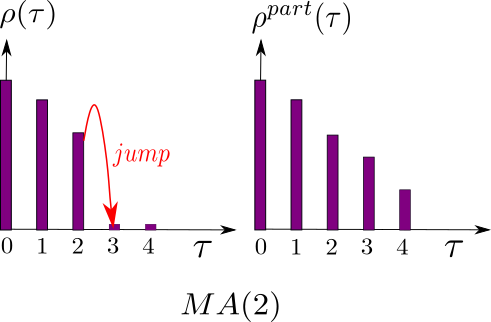
\includegraphics[width=3in]
{time-arma/ma-2-ac-pac.png}
\caption{
Plot of auto-correlation function (ACorrF)
$\rho(\tau)$
and partial auto-correlation
function (PACorrF) $\rho^{part}(\tau)$
for an instance
of $MA(2)$. Note
that $\rho(\tau)$
vanishes for $\tau>2$.
} 
\label{fig-ma-2-ac-pac}
\end{figure}


\begin{claim}
If $\tseries{\rvy_t}$
is an $AR(p)$ t-series, then
$\gamma^{part}(\tau)=0$  for all $\tau>p$.
\end{claim}
\proof


Let 

\beq
\ul{\xi}=\rvy_{\leq t},
\rvy_{t+\tau}
\eeq
Recall that

\beqa
\gamma^{part}(\tau)
&=&
\av{\rvy_t, \rvy_{t+\tau}}_{|\xi}
\\
&=&
\av{\rvy_t \;\rvy_{t+\tau}}_{|\xi}
-\av{\rvy_t}_{|\xi}
\av{ \rvy_{t+\tau}}_{|\xi}
\\
&=&
\av{\rvy_t\; \rvy_{t+\tau}}_{|\xi}
\eeqa
Define

\beq
Z_{(t, t+\tau)}=\indi(
\rvy_{(t, t+\tau)}=0)
\eeq
Hence, the operator
$Z_{(t, t+\tau)}$
sets
 all $\rvy_{t'}$
with $t<t'<t+\tau$ equal to zero.
Note that we can express the PACov as

\beq
\gamma^{part}(\tau)=
\av{Z_{(t, t+\tau)}\;(
\rvy_{t}\;\rvy_{t+\tau})}
\;.
\eeq
Since

\beqa
\rvy_{t+\tau}
&=&
\sum_{j=1}^p\alp_{j}\rvy_{t+\tau-j}
+\rvn_{t+\tau}
\\
&=&
\alp_{p}\rvy_{t+\tau-p}
+
\ldots
+ \alp_{2}\rvy_{t+\tau-2}
+\alp_{1}\rvy_{t+\tau-1}
+\rvn_{t+\tau}
\;,
\eeqa
we get

\beq
Z_{(t, t+\tau)}\rvy_{t+\tau}
=
\rvn_{t+\tau} \;\;\;\text{if $\tau> p$}
\;.
\eeq
Hence, for $\tau>p$,

\beq
\gamma^{part}(\tau)=
\av{\rvy_t\;\rvn_{t+\tau}}
=0
\eeq
\qed

Fig.\ref{fig-ar-2-tau-123}
gives a graphical proof,
using
bnets and the
d-separation
theorem,
that 
for an $AR(2)$
t-series, $\gamma^{part}(\tau)=0$
for $\tau>2$.
As a consequence of this,
a plot of $\gamma^{part}(\tau)$
versus $\tau$
for a typical $AR(2)$
t-series looks like
 Fig.\ref{fig-ar-2-ac-pac}.
 


\begin{figure}[h!]
$$
\begin{array}{ll}
\tau=1&
\xymatrix@C=36px{
\cdots
\rvn_{t-2}
&\rvn_{t-1}
&\rvn_t\ar[d]_1
&\rvn_{t+1}\ar[d]_1
&\rvn_{t+2}
&\rvn_{t+3}
\cdots
\\
\cdots
\rvy_{t-2}
\ar@/_1pc/[rr]_{\alp_2}
&\rvy_{t-1}
\ar@/_1pc/[rr]_{\alp_2}
\ar[r]_{\alp_1}
&{\color{red}\rvy_t}
\ar[r]_{\alp_1}
&{\color{red}\rvy_{t+1}}
&\rvy_{t+2}
&\rvy_{t+3}
\cdots
}
\\
\\
\tau=2&
\xymatrix@C=36px{
\cdots
\rvn_{t-2}
&\rvn_{t-1}
&\rvn_t\ar[d]_1
&\rvn_{t+1}
&\rvn_{t+2}\ar[d]_1
&\rvn_{t+3}
\cdots
\\
\cdots
\rvy_{t-2}
\ar@/_1pc/[rr]_{\alp_2}
&\rvy_{t-1}
\ar[r]_{\alp_1}
&{\color{red}\rvy_t}
\ar@/_1pc/[rr]_{\alp_2}
&*+[F]{\rvy_{t+1}}
\ar[r]_{\alp_1}
&{\color{red}\rvy_{t+2}}
&\rvy_{t+3}
\cdots
}
\\
\\
\tau=3&
\xymatrix@C=36px{
\cdots
\rvn_{t-2}
&\rvn_{t-1}
&\rvn_t\ar[d]_1
&\rvn_{t+1}
&\rvn_{t+2}
&\rvn_{t+3}\ar[d]_1
\cdots
\\
\cdots
\rvy_{t-2}
\ar@/_1pc/[rr]_{\alp_2}
&\rvy_{t-1}
\ar[r]_{\alp_1}
&{\color{red}\rvy_t}
&*+[F]{\rvy_{t+1}}
\ar@/_1pc/[rr]_{\alp_2}
&*+[F]{\rvy_{t+2}}
\ar[r]_{\alp_1}
&{\color{red}\rvy_{t+3}}
\cdots
}
\end{array}
$$
\caption{$AR(2)$ bnet.
For clarity, we show only arrows 
entering nodes
$\rvy_t$ and $\rvy_{t+\tau}$
for $\tau=1,2,3$.
Boxed nodes are
in set $\rvy_{(t, t+\tau)}$.
They are conditioned on, so 
information can't flow through them
to node $\rvy_{t+\tau}$
by the d-separation theorem.
}
\label{fig-ar-2-tau-123}
\end{figure}

\begin{figure}[h!]
\centering
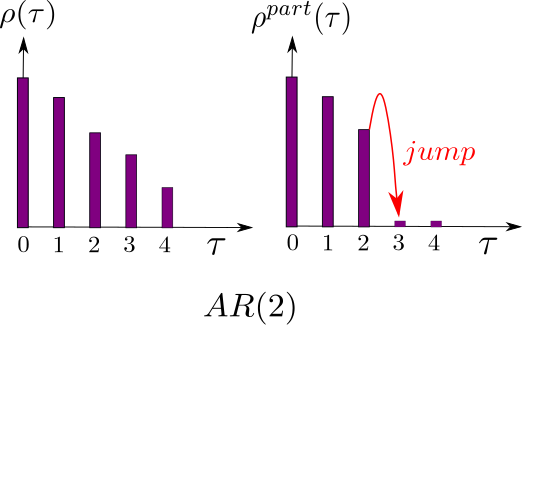
\includegraphics[width=3in]
{time-arma/ar-2-ac-pac.png}
\caption{
Plot of auto-correlation function (ACorrF)
$\rho(\tau)$
and partial auto-correlation
function (PACorrF) $\rho^{part}(\tau)$
for an instance
of $AR(2)$. Note
that $\rho^{part}(\tau)$
vanishes for $\tau>2$.
} 
\label{fig-ar-2-ac-pac}
\end{figure}

\begin{table}[h!]
\centering
\begin{tabular}{|l|l|l|}
\hline
 & ACorr & PACorr \\ \hline
$AR(p)$ & \cellcolor[HTML]{FDF2FD}tapers off &
 \cellcolor[HTML]{EBF6E2}jumps to zero for $\tau>p$ \\ \hline
$MA(q)$ & \cellcolor[HTML]{EBF6E2}jumps to zero for $\tau>q$ &
 \cellcolor[HTML]{FDF2FD}tapers off \\ \hline
\end{tabular}
\caption{Detecting $AR(p)$ and $MA(q)$ using auto-correlation and partial auto-correlation.}
\label{tab-ar-ma-diff}
\end{table}

\section{Generating function
of auto-correlation}

\begin{claim}
\label{claim-az-azinv}
If
\beq
\alp(z)=\sum_{\tau=-\infty}^\infty
\alp_\tau z^\tau
\eeq
then 

\beq
\alp(z)\alp(z^{-1})=
\sum_{\tau=-\infty}^\infty z^\tau
\sum_{j=-\infty}^\infty
\alp_{j}\alp_{j+\tau}
\eeq
\end{claim}
\proof

\beqa
\alp(z)\alp(z^{-1})
&=&
\sum_{j'=-\infty}^\infty z^{j'}\alp_{j'}
\sum_{j=-\infty}^\infty z^{-j}\alp_{j}
\\
&=&
\sum_{\tau=-\infty}^\infty
\sum_{j'=-\infty}^\infty 
\sum_{j=-\infty}^\infty 
z^\tau
\alp_{j'}\alp_{j}\delta(j'-j,\tau)
\\
&=&
\sum_{\tau=-\infty}^\infty z^\tau
\sum_{j=-\infty}^\infty
\alp_{j}\alp_{j+\tau}
\eeqa
\qed

As an example
of this claim, note that
\beq
(\alp_0+\alp_1z)(\alp_0+\alp_1 z^{-1})
=
\alp_0\alp_1 z^{-1}+ 
(\alp_0^2 +\alp_1^2) +\alp_0\alp_1z
\eeq


\begin{claim}
If $\tseries{\rvy_t}$ is an $AR(p)$ t-series,
then
\beq
\tilde{\gamma}(z) =
\alp'(z)\s^2\alp'(z^{-1})
\eeq
\end{claim}
\proof
 Left to reader.
See Claim 
\ref{claim-az-azinv}.
\qed

\begin{claim}
If $\tseries{\rvy_t}$ is an $MA(q)$
 t-series, then
\beq
\tilde{\gamma}(z) =
\nu(z)\s^2 \nu(z^{-1})
\eeq
\end{claim}
\proof

\beq
\rvy_t = \sum_{j=-\infty}^\infty\nu_{j}\rvn_{t-j}
\eeq

\beqa
\tilde{\gamma}(z)&=&
\sum_{\tau=-\infty}^\infty \av{\rvy_0, \rvy_{\tau}} z^\tau
\\
&=&
\sum_{\tau=-\infty}^\infty z^\tau
\sum_{j=-\infty}^\infty
\sum_{j'=-\infty}^\infty\nu_j\nu_{j'}
\underbrace{\av{
\rvn_{-j}, \rvn_{\tau-j'}}}_{\s^2\delta(j', \tau + j)}
\\
&=&\s^2
\sum_{\tau=-\infty}^\infty z^\tau
\sum_{j=-\infty}^\infty\nu_j\nu_{j+\tau}
\eeqa
Now use Claim 
\ref{claim-az-azinv}.
\qed

\begin{claim}
If $\tseries{\rvy_t}$ is an $ARMA(p,q)$
 t-series, then
\beq
\tilde{\gamma}(z) =
\alp'(z)
\nu(z)
\s^2
\nu(z^{-1})
\alp'(z^{-1})
\eeq
\end{claim}
\proof
 Left to reader.
See Claim 
\ref{claim-az-azinv}.
\qed

\section{Impulse Response}
The
derivatives

\beq
IR_\tau= \pder{y_{t+\tau}}{n_t}
\eeq
are 
 called {\bf impulse responses}
or {\bf dynamic multipliers}.
Note
that this derivative 
depends on $\tau$ but not $t$
by w-stationarity.
A plot of $IR_\tau$
versus $\tau$ is called 
the {\bf Impulse Response Function (IRF)}.
Examples:

\begin{itemize}
\item
\begin{claim}
For $MA(q)$,

\beq
\pder{y_{t+\tau}}{n_t}=\nu_\tau
\indi(0\leq \tau \leq q)
\label{eq-ir-ma-q}
\eeq
where $\nu_0=1$.
(See
Fig.\ref{fig-imp-res-nu-2})
\end{claim}
\proof
\beq
\rvy_{t+\tau}=\sum_{j=0}^q\nu_j\rvn_{t+\tau-j}
\eeq
so Eq.(\ref{eq-ir-ma-q}) follows.
\qed

\item
\begin{claim}
For $AR(1)$,

\beq
\pder{y_{t+\tau}}{n_t}=(\alp_1)^\tau
\indi(\tau \geq 0).
\label{eq-ir-ar-1}
\eeq
(See Fig.\ref{fig-imp-res-ar-1})
\end{claim}

\proof
\beq
(1-\alp_1\calb)\rvy_{t+\tau}=\rvn_{t+\tau}
\eeq
Therefore, using 
the Taylor expansion Eq.(\ref{eq-binomial-expan}), 
\beqa
\rvy_{t+\tau} 
&=& 1 +\sum_{j=1}^\infty\alp_1^j\calb^j\rvn_{t+\tau}
\\
&=&
1 +\sum_{j=1}^\infty\alp_1^j\rvn_{t+\tau-j}
\eeqa
so Eq.(\ref{eq-ir-ar-1}) follows.
\qed
\end{itemize}
In general, 
$IR_\tau$
equals 
a sum 
over 
paths
from $\rvn_t$ to
$\rvy_{t+\tau}$.
Each path
contributes the
product
of the weights
of all the arrows in the path.



\begin{figure}[h!]
$$
\xymatrix{
\cdots
\rvn_{t}\ar[drr]_{\nu_2}
&\rvn_{t+1}
&\rvn_{t+2}\cdots
\\
\cdots
\rvy_{t}
&\rvy_{t+1}
&\rvy_{t+2}\cdots
}$$
\caption{Pictorial
representation of impulse
response $IR_2=\nu_2$
for a $MA(q)$ t-series with $q\geq 2$.}
\label{fig-imp-res-nu-2}
\end{figure}

\begin{figure}[h!]
$$
\xymatrix{
\cdots
\rvn_{t}\ar[d]_1
&\rvn_{t+1}
&\rvn_{t+2}\cdots
\\
\cdots
\rvy_{t}\ar[r]_{\alp_1}
&\rvy_{t+1}\ar[r]_{\alp_1}
&\rvy_{t+2}\cdots
}$$
\caption{Pictorial
representation of impulse
response $IR_2=\alp_1^2$
for an $AR(1)$ t-series.}
\label{fig-imp-res-ar-1}
\end{figure}





\section{$AR(p)$ and Yule-Walker
 equations}
\begin{claim} (Yule-Walker equations)
If $\tseries{\rvy_t}$ is an $AR(p)$ t-series,

\beq
\gamma_\tau=
\sum_{j=1}^p\gamma_{\tau-j}\alp_j
+
\s^2\delta(\tau,0)
\label{eq-yule-walker}
\eeq
for all $\tau\in \ZZ$,
where we are abbreviating 
$\gamma(j)=\gamma_j$ for all $j$.
\end{claim}
\proof 

Recall that
\beq
\rvy_\tau = 
\sum_{j=1}^p \rvy_{\tau-j}\alp_j
+
\rvn_\tau
\eeq
Therefore

\beq
\underbrace{
\av{\rvy_0, \rvy_\tau}
}_{\gamma_\tau}
=
\sum_{j=1}^p
\underbrace{
\av{\rvy_0,
\rvy_{\tau-j}}
}_{\gamma_{\tau-j}}
\alp_j
+
\underbrace{
\av{\rvy_0, \rvn_\tau}
}_{\s^2\delta(\tau,0)}
\eeq
\qed

\begin{figure}[h!]
$$
\xymatrix@C=36px{
\cdots
\rvc_{\tau-4}
&\rvc_{\tau-3}
&\rvc_{\tau-2}
&\rvc_{\tau-1}
&\rvc_\tau\ar[d]^{\s^2\delta(\tau,0)}
&\rvc_{\tau+1}
&\rvc_{\tau+2}
\cdots
\\
\cdots
\ul{\gamma}_{\tau-4}
&\ul{\gamma}_{\tau-3}\ar@/_2pc/[rrr]_{\alp_3}
&\ul{\gamma}_{\tau-2}\ar@/_1pc/[rr]_{\alp_2}
&\ul{\gamma}_{\tau-1}\ar[r]_{\alp_1}
&{\color{red}\ul{\gamma}_\tau}
&\ul{\gamma}_{\tau+1}&\ul{\gamma}_{\tau+2}
\cdots
}$$
\caption{Bnet representing 
Yule-Walker (Christmas Walker)
Eqs.(\ref{eq-yule-walker})
with $p=3$.
For clarity, we show only arrows
 entering node
 $\ul{\gamma}_\tau$.
The full bnet has the same
structural  pattern of incoming arrows
(including the  $\alp_j$)
for each node
$\gamma_{\tau'}$ for all $\tau'$.}
\label{fig-bnet-yule-walker}
\end{figure}

Fig.\ref{fig-bnet-yule-walker}
shows a bnet 
for the
Yule-Walker 
Eqs.(\ref{eq-yule-walker}.
The TPMs,
printed in blue, for the
$\tau$ time slice of that
bnet, are
as follows:

\beq\color{blue}
P(\gamma_\tau)=
\indi\left(\gamma_\tau=
\text{ See Eq.(\ref{eq-yule-walker})}
\right)
\eeq

\beq\color{blue}
P(c_\tau)=
\indi(c_\tau=\s^2\delta(\tau, 0))
\eeq


The Yule-Walker 
Eqs.(\ref{eq-yule-walker})
imply that


\beq
\underbrace{
\left[
\begin{array}{c}
\gamma_1 \\ \gamma_2 \\ \vdots\\ \gamma_p
\end{array}
\right]
}_{\gamma^p}
=
\underbrace{
\left[
\begin{array}{ccccc}
\gamma_0 & \gamma_{-1} &\gamma_{-2}& \hdots&\gamma_{1-p}
\\
\gamma_{1} & \gamma_{0} &\gamma_{-1}&\hdots&\gamma_{2-p}
\\
\vdots
\\
\gamma_{p-1} & \gamma_{p-2} &\gamma_{p-3}&\hdots&\gamma_{0}
\end{array}
\right]
}_{\Gamma}
\underbrace{
\left[
\begin{array}{c}
\alp_1 \\ \alp_2 \\ \vdots\\ \alp_p
\end{array}
\right]
}_{\alp^p}
\eeq
Hence

\beq
\gamma^p=\Gamma \alp^p
\;.
\eeq
If $\Gamma$
is invertible,

\beq
\alp^p=\Gamma^{-1}\gamma^p
\;.
\eeq
Once we know $\alp^p$,
we can solve for $\s^2$ 
\beq
\gamma_0=\sum_{j=1}^p\gamma_{-j}\alp_j
+ \s^2
\;,
\eeq
i.e., 
Eq.(\ref{eq-yule-walker}) for $\tau=0$.



\section{Forecasting}




Before 
submerging
the reader
in the messy details
of t-series forecasting,
and running
the risk of quickly losing him/her,
let me explain to the reader that
what we are about
to do in this section, is, in the final 
analysis, quite trivial,
and boils down to 
solving simple
systems
of linear equations.
That is all there is to it!!
How hard can that be?
In reading this section,
don't lose sight of that fact and
you'll be okay.

Suppose 
$\tseries{\rvy_t}$
is an $AR(\infty)$ t-series. For $\tau>0$,
the ``orthogonal projection" 
$\rvy_{t+\tau}|\rvy_{\leq t}$
is defined as the 
linear combination of $\rvy_{\leq t}$
obtained by doing
Linear Regression
with x-variables
$\rvy_{\leq t}$
and y-variable
$\rvy_{t+\tau}$. Thus

\beq
E\left[\rvy_{t+\tau}|\rvy_{\leq t}\right]
=
E_{|\rvy_{\leq t}}[\rvy_{t+\tau}]
\eeq
and

\beqa
Var\left[\rvy_{t+\tau}|\rvy_{\leq t}\right]&=&
E\left[
\left(\rvy_{t+\tau}|\rvy_{\leq t}
-E[\rvy_{t+\tau}|\rvy_{\leq t}]
\right)^2\right]
\\
&=&
Var_{|\rvy_{\leq t}}[\rvy_{t+\tau}]
\;.
\eeqa
For example, for $\tau=1$,


\beq 
\rvy_{t+1} = \sum_{j=1}^p \alp_j \rvy_{t+1-j}
+ \rvn_{t+1}
\eeq

\beq 
\rvy_{t+1}|\rvy_{\leq t} = 
\sum_{j=1}^p \alp_j \rvy_{t+1-j}
\eeq

\beq
\rvy_{t+1}-\rvy_{t+1|\rvy{\leq t}}=\rvn_{t+1}
\eeq

\beqa
E\left[\rvy_{t+1}|\rvy_{\leq t}\right]&=&
E_{|\rvy_{\leq t}}[\rvy_{t+1}]
\\
&=&0
\eeqa

\beqa
Var\left[
\rvy_{t+1}|\rvy_{\leq t}\right]
&=&
Var_{|\rvy_{\leq t}}[\rvy_{t+1}]
\\
&=& \s^2
\eeqa

If $\tseries{\rvy_t}$
is an $AR(\infty)$
t-series and $\tau>0$, 
by {\bf forecasting} $\rvy_{t+\tau}|\rvy_{\leq t}$ ,
we will mean
finding $\rvy_{t+\tau}|\rvy_{\leq t}$,
given
$y_{\leq t}$
as input data
or some other input data
from which $y_{\leq t}$
can be derived.
Fig.\ref{fig-forecasting-cases}
illustrates 3 types 
of input 
data that we will consider
next.



Note that if $\tseries{\rvy_t}$
is an $AR(\infty)$
t-series, 
then $\alp^-(\calb)\rvy_t=n_t$.
Thus, $\rvn_{\leq t}$
can be expressed in terms 
of $\rvy_{\leq t}$,
yielding a function 
$\rvn_{\leq t}(\rvy_{\leq t})$.
If the operator
$\alp^-(\calb)$
is invertible,
the opposite is also true: $\rvy_{\leq t}$
can be expressed in terms
of $\rvn_{\leq t}$,
yielding a function 
$\rvy_{\leq t}(\rvn_{\leq t})$.
Thus, 

\beq
\rvy_{t+\tau}|\rvy_{\leq t}=
\rvy_{t+\tau}|\rvy_{\leq t}(\rvn_{\leq t})=
\rvy_{t+\tau}|\rvn_{\leq t}
\eeq

We've
seen that
 if we 
assume invertibility
of $\alp^-(\calb)$, then,
in order 
to forecast $\rvy_{t+\tau}|\rvy_{\leq t}$,
we have the option
of considering $\tseries{\rvy_t}$ to be
either an $AR(\infty)$
or an $MA(\infty)$
t-series. We will assume
the latter,
because this
simplifies 
the algebra
necessary to calculate
both
$\rvy_{t+\tau}|\rvy_{\leq t}$
and its 
variance.


\newcommand{\yLt}[0]
{given $\rvy_{\leq t}$}


\newcommand{\ynAPPROX}[0]
{given $\rvy_{\leq t}$, but,
 for some $m>0$,
$\rvy_{\leq t-m}\approx 0$ (approximation)}

\newcommand{\gammaEXACT}[0]
{given $\gamma_{[0,m-1]}$
and $\gamma^{part}_{[\tau,\tau+ m-1]}$}


\begin{figure}[h!]
$$
\begin{array}{c}
\fbox{\text{\color{red}(a) \yLt}}
\\
\xymatrix{
\cdots
\rvn_{t-2}\ar[drr]
&\rvn_{t-1}\ar[dr]
&\rvn_t\ar[d]
&\rvn_{t+1}
&\cdots
&\rvn_{t+\tau}
\cdots
\\
\cdots
{\color{red}\rvy_{t-2}}
&{\color{red}\rvy_{t-1}}
&{\color{red}\rvy_t}
&\rvy_{t+1}
&\cdots
&\rvy_{t+\tau}
\cdots
}
\\
\\
\\
\fbox{\text{\color{red}(b) \ynAPPROX}}
\\
\xymatrix@C=10px{
\cdots
\rvn_{t-m-1}\ar[drrrr]
&\rvn_{t-m}\ar[drrr]
&\rvn_{t-m+1}\ar[drr]
&\cdots
&\rvn_{t}\ar[d]
&\rvn_{t+1}
&\cdots
&\rvn_{t+\tau}
\cdots
\\
\cdots
{\color{red}\rvy_{t-m-1}=0}
&{\color{red}\rvy_{t-m}=0}
&{\color{red}\rvy_{t-m+1}}
&\cdots
&{\color{red}\rvy_{t}}
&\rvy_{t+1}
&\cdots
&\rvy_{t+\tau}
\cdots
}
\\
\\
\\
\fbox{\color{red}(c) \gammaEXACT}
\\
\xymatrix@C=10px{
\cdots
\rvy_{t-m-1}
&\rvy_{t-m}
&\rvy_{t-m+1}
&\rvy_{t-m+2}
&\cdots
&\rvy_{t}\ar@[red]@/_3pc/@{-}[lll]_\gamma
\ar@[red]@/_1.5pc/@{-}[ll]_\gamma
\ar@[red]@(ul,ur)[]^\gamma
&\rvy_{t+1}
&\cdots
&\rvy_{t+\tau}
\ar@[red]@/^1.5pc/@{--}[lll]^{\gamma^{part}}
\ar@[red]@/^3pc/@{--}[lllll]^{\gamma^{part}}
\ar@[red]@/^4.5pc/@{--}[llllll]^{\gamma^{part}}
\cdots
}
\end{array}
$$
\caption{Bnet for 
$MA(\infty)$
for forecasting
$\rvy_{t+\tau}|\rvy_{\leq t}$.
Input data in red.
For clarity, we show
 only the arrows entering
node $\rvy_t$.}
\label{fig-forecasting-cases}
\end{figure}

\begin{enumerate}[(a)]
\item
{\bf find $\rvy_{t+\tau}|y_{\leq t}$
\yLt}

Suppose $\tseries{\rvy_t}$
is an $MA(\infty)$ t-series. Then




\beqa
\rvy_{t+\tau}
&=&
\sum_{j=0}^\infty
\nu_{j}\rvn_{t+\tau-j}
\\
&=&
\underbrace{
\sum_{j=0}^{\tau-1}
\nu_{j}\rvn_{t+\tau-j}
}_{\color{red}\rvy_{t+\tau}-
\rvy_{t+\tau}|y_{\leq t}
}
+
\underbrace{
\sum_{j=\tau}^\infty
\nu_{j}\rvn_{t+\tau-j}
}_{\rvy_{t+\tau}|y_{\leq t}}
\eeqa

\beq
\rvy_{t+\tau}|y_{\leq t}=
\sum_{j=\tau}^\infty
\nu_{j}\rvn_{t+\tau-j}
\label{eq-wk-simple}
\eeq


\beq
E_{|y_{\leq t}}[\rvy_{t+\tau}]=
E[\rvy_{t+\tau}|y_{\leq t}]
=0\footnote{Remember
that $\rvy_t$ has zero mean by definition.
$Y_t=y_t+\mu$
for some time
independent constant $\mu$.}
\eeq

\beqa
\av{\rvy_{t+\tau}\rvy_
{t+\tau}}_{|y_{\leq t}}
&=&
\av{
{\color{red}
\rvy_{t+\tau}-
\rvy_{t+\tau}|y_{\leq t}},\;\;
\rvy_{t+\tau}-
\rvy_{t+\tau}|y_{\leq t}}
\\
&=&
\sum_{j=0}^{\tau-1}
\nu_j^2
\eeqa

\begin{figure}[h!]
$$
\begin{array}{ll}
\tau=1&
\xymatrix@C=36px{
\cdots
\rvn_{t-2}
&\rvn_{t-1}
\ar[drr]_(.3){\nu_2}
&\rvn_t
\ar[dr]_(.3){\nu_1}
&\rvn_{t+1}\ar@[green][d]^>1
&\rvn_{t+2}
&\rvn_{t+3}
\cdots
\\
\cdots
\rvy_{t-2}
&\rvy_{t-1}
&{\color{red}\rvy_t}
&{\color{red}\rvy_{t+1}}
&\rvy_{t+2}
&\rvy_{t+3}
\cdots
}
\\
\\
\tau=2&
\xymatrix@C=36px{
\cdots
\rvn_{t-2}
&\rvn_{t-1}
&\rvn_t\ar[drr]_(.3){\nu_2}
&\rvn_{t+1}\ar@[green][dr]_(.3){\nu_1}
&\rvn_{t+2}\ar@[green][d]^>1
&\rvn_{t+3}
\cdots
\\
\cdots
\rvy_{t-2}
&\rvy_{t-1}
&{\color{red}\rvy_t}
&{\rvy_{t+1}}
&{\color{red}\rvy_{t+2}}
&\rvy_{t+3}
\cdots
}
\\
\\
\tau=3&
\xymatrix@C=36px{
\cdots
\rvn_{t-2}
&\rvn_{t-1}
&\rvn_t
&\rvn_{t+1}\ar@[green][drr]_(.3){\nu_2}
&\rvn_{t+2}\ar@[green][dr]_(.3){\nu_1}
&\rvn_{t+3}\ar@[green][d]^>1
\cdots
\\
\cdots
\rvy_{t-2}
&\rvy_{t-1}
&{\color{red}\rvy_t}
&{\rvy_{t+1}}
&{\rvy_{t+2}}
&{\color{red}\rvy_{t+3}}
\cdots
}
\end{array}
$$
\caption{$MA(2)$ bnet.
For clarity, we show only arrows 
entering node $\rvy_{t+\tau}$
for $\tau=1,2,3$.
Green arrows
originate at a time after
time $t$.
}
\label{fig-ma-2-tau-123-redux}
\end{figure}

For $MA(q)$,
because $\nu_j=0$ for $j>q$, 
this reduces to

\beq
\rvy_{t+\tau}|y_{\leq t}=
\indi(\tau\leq q)
\sum_{j=\tau}^q
\nu_{j}\rvn_{t+\tau-j}
\eeq

\beq
E_{|y_{\leq t}}[\rvy_{t+\tau}]=
E[\rvy_{t+\tau}|y_{\leq t}]=0
\eeq


\beqa
\av{\rvy_{t+\tau},\rvy_
{t+\tau}}_{|y_{\leq t}}=
\sum_{j=0}^{\min(\tau-1, q)}
\nu_j^2
\label{eq-ma-2-forecast-noise}
\eeqa
Eq.(\ref{eq-ma-2-forecast-noise})
is motivated by  
Fig.\ref{fig-ma-2-tau-123-redux}).
Only
the green arrows 
entering $\rvy_{t+\tau}$
and originating
in a node  $\rvn_{t'}$ with
$t'>t$
contribute to the right hand side
of 
Eq.(\ref{eq-ma-2-forecast-noise}). 


Thus, the mean 
of $\rvy_{t+\tau}$
can be
predicted to
remain zero
for all $\tau>0$ (forever).
The error
in that prediction increases with $\tau$
until
$\tau$ reaches $q$.
After that, the error remains constant.

Note that

\beqa
\rvy_{t+\tau}|y_{\leq t}
&=&
\sum_{j=\tau}^{\infty}
\nu_j\rvn_{t+\tau-j}
\\
&=&
\sum_{j=\tau}^{\infty}
\nu_j\calb^{j-\tau}\rvn_{t}
\\
&=&
\left[
\sum_{j=0}^{\infty}
\nu_j\calb^{j-\tau}\right]_{\calb^{\geq 0}}\rvn_{t}
\\
&=&
\left[\calb^{-\tau}
\nu(\calb)\right]_{\calb^{\geq 0}}
\rvn_{t}
\label{eq-wk-fancy}
\eeqa
$\calb^{\geq 0}$ means only
the non-negative powers of
$\calb$ are kept.
Eq.(\ref{eq-wk-fancy})
is just Eq.(\ref{eq-wk-simple})
in fancy notation.

In $MA(\infty)$, 
if $\nu(\calb)$ is invertible,
then

\beq
\rvn_t
=
\nu(\calb)^{-1}  \rvy_t
\eeq
so


\beq
\boxed{
\rvy_{t+\tau}|y_{\leq t}=
\call_{WK}  \rvy_t}
\label{eq-wk-pred-formula}
\eeq

where
\beq
\call_{WK}=
\left[\calb^{-\tau}
\nu(\calb)\right]_{\calb^{\geq 0}}
\nu(\calb)^{-1}
\eeq

Eq.(\ref{eq-wk-pred-formula})
is called the {\bf Wiener-Kolgomorov
 prediction formula (WKPF)}.
Next, we apply WKPF
to $AR(1)$ and $MA(1)$
as examples of its usage.

\begin{itemize}
\item  $AR(1)$

\beq
\underbrace{(1-\alp_1\calb)}
_{\nu(\calb)^{-1}}
\rvy_t = \rvn_t
\eeq

\beq
\rvy_t = \underbrace{\left[\sum_{j=0}^\infty
(\alp_1\calb)^j\right]}
_{\nu(\calb)}
\rvn_t
\eeq

\beq
\nu_j=(\alp_1)^j
\eeq

\beq
\left[\calb^{-\tau}
\nu(\calb)\right]_{\calb^{\geq 0}}
=
(\alp_1)^\tau \nu(\calb)
\eeq

\beq
\rvy_{t+\tau}|y_{\leq t}=
(\alp_1)^\tau \rvy_t
\eeq
Hence, $\rvy_{t+\tau}|y_{\leq t}$
decreases geometrically
as $\tau$ grows.

\item $MA(1)$

\beq
\rvy_t=
\underbrace{ (1+\nu_1\calb)
}_{\nu(\calb)}
\rvn_t
\eeq

\beq
\left[\calb^{-\tau}
\nu(\calb)\right]_{\calb^{\geq 0}}
=
\delta(\tau,1)\nu_1
\eeq

\beqa
\rvy_{t+\tau}|y_{\leq t}
&=&
\delta(\tau,1)
\nu_1
\underbrace{\left[\sum_{j=0}^\infty
(-\nu_1\calb)^j \right]}_{
\nu(\calb)^{-1}}
\rvy_t
\\
&=&
\delta(\tau,1)
\nu_1\rvn_t
\eeqa

\end{itemize}



\item {\bf find $\rvy_{t+\tau}|y_{\leq t}$
\ynAPPROX}

\beqa
\rvy_{t+\tau}|
\rvy_{\leq \tau}
&\approx&\indi(\rvy_{\leq t-m}=0)
\call_{WK}
\rvy_t
\eeqa



\item {\bf find $\rvy_{t+\tau}|y_{\leq t}$
\gammaEXACT}

\beq
\rvy_{t+\tau}|\rvy_{\leq t} = 
\sum_{j=0}^{m-1} \rvy_{t-j}\beta_j
\label{eq-pseudo-yule-target}
\eeq

Suppose that $k\in \ZZ_{[0,m-1]}$.

Note that 

\beq
\rvy_{t-k}|\rvy_{\leq t}=\rvy_{t-k}
\;.
\eeq


\beq
\underbrace{
\av{\rvy_{t-k}|\rvy_{\leq t}\;\;,\;\;
\rvy_{t+\tau}|\rvy_{\leq t}}
}_{\gamma^{part}_{\tau+k}} = 
\sum_{j=0}^{m-1} 
\underbrace{
\av{\rvy_{t-k}\;\;,\;\;\rvy_{t-j}}
}_{\gamma_{k-j}}
\beta_j
\eeq

{\renewcommand{\arraystretch}{1.5}
\beq
\left[
\begin{array}{c}
\gamma_{\tau}^{part} 
\\ \gamma_{\tau+1}^{part} \\ \vdots\\
 \gamma_{\tau+m-1}^{part}
\end{array}
\right]
=
\underbrace{
\left[
\begin{array}{ccccc}
\gamma_0 & \gamma_{-1} &\gamma_{-2}& \hdots&\gamma_{1-m}
\\
\gamma_{1} & \gamma_{0} &\gamma_{-1}&\hdots&\gamma_{2-m}
\\
\vdots
\\
\gamma_{m-1} & \gamma_{m-2} &\gamma_{m-3}&\hdots&\gamma_{0}
\end{array}
\right]
}_{\Gamma}
\underbrace{
\left[
\begin{array}{c}
\beta_0 \\ \beta_1 \\ \vdots\\ \beta_{m-1}
\end{array}
\right]
}_{\beta^m}
\label{eq-pseudo-yule}
\eeq}
Solve Eq.(\ref{eq-pseudo-yule})
for $\beta^m$
and plug $\beta^m$
into Eq.(\ref{eq-pseudo-yule-target}).

\end{enumerate}


\section{Model Learning}

{\bf Box-Jenkins Method}

\begin{enumerate}
\item {\bf Filtering Data (FD)}

Removing trends and periodicity 
(seasonality) via
differencing, 
so as to achieve a w-stationary
t-series. We deal with FD in Section 
\ref{sec-time-arma-diff}.


\item {\bf Model Selection}

Finding best possible $p, q$
for $ARMA(p,q)$
using various
statistical tests and metrics.

\item {\bf Parameter Learning (PL)}

Finding best possible coefficients
$\alp_j$ and $\nu_j$.
We deal with
PL in Section 
\ref{sec-time-arma-param-learn}.


\item {\bf Testing}

Measuring the goodness of fit.

\end{enumerate}

\section{Differencing and
$ARIMA(p,d,q)$}\label{sec-time-arma-diff}

Let  $\alp\in(0,1)$.
We say that $\tseries{\rvs_t}$
is a {\bf Simple Exponential
 Smoothing (SES) t-series}
if it satisfies 

\beq
s_t= (1-\alp) s_{t-1}+ \alp x_t
\label{eq-ses-tseries}
\eeq


\begin{figure}[h!]
$$
\xymatrix{
\cdots
\rvx_{t-2}\ar[d]_\alp
&\rvx_{t-1}\ar[d]_\alp
&\rvx_t\ar[d]_\alp
&\rvx_{t+1}\ar[d]_\alp
\cdots
\\
\cdots
\rvs_{t-2}\ar[r]^{1-\alp}
&\rvs_{t-1}\ar[r]^{1-\alp}
&\rvs_t\ar[r]^{1-\alp}
&\rvs_{t+1}
\cdots
}$$
\caption{Bnet for Simple Exponential 
Smoothing t-series.  $\alp\in(0,1)$}
\label{fig-simple-ex-smoo}
\end{figure}

A SES t-series can be represented by
the bnet of Fig.\ref{fig-simple-ex-smoo}.
The TPM, printed in blue,
for node $\rvs_t$,
is as follows

\beq\color{blue}
P(s_t)=\indi(s_t=\text{ see 
Eq.(\ref{eq-ses-tseries}))}
\eeq

One has
\beq
(1 - (1-\alp)\calb)\rvs_t= \alp\rvx_t
\eeq
so

\beqa
\rvs_t &=&
\frac{\alp}{1 -(1-\alp)\calb}\rvx_t
\\
&=&
\alp\sum_{j=0}^\infty
(1-\alp)^j\calb^j\rvx_t\;\;\text{ 
(by Eq.(\ref{eq-binomial-expan}))}
\label{eq-expand-simple-smoo}
\eeqa

Note from 
Fig.\ref{fig-simple-ex-smoo}
and Eq.(\ref{eq-expand-simple-smoo})
that each shock $\rvx_{t-j}$
with $j>0$
contributes to 
$\rvs_t$ 
proportionally
to the product
$\alp (1-\alp)^j$ of 
arrow weights in the  path
from $\rvx_{t-j}$
to $\rvs_t$.
For example,
$\rvx_{t-2}$
contributes to $\rvs_t$
in the proportion $\alp (1-\alp)^2$.
The contributions of $\rvx_{t-j}$
to $\rvs_t$
decrease geometrically as the lag
$j$ increases. 

Henceforth, we  will 
abbreviate
``{\bf differencing}" by ``
{\bf diff}".

\begin{itemize}
\item
{\bf First order diff
operator}
\beq
\Delta x_t = x_t-x_{t-1}= (1-\calb)x_t
\eeq


 Seasonal first order diff:
\beq
\Delta_{sea} x_t = x_t-x_{t-ts}
\eeq
where $ts$ is length of season.

\item
{\bf Second order diff
operator}
\beqa
\Delta^2 x_{t} &=& \Delta x_{t}-
\Delta x_{t-1}
\\
&=&
x_{t}-2 x_{t-1} + x_{t-2}
\\
&=&
(1-2\calb+\calb^2)x_{t}
\\
&=&
(1-\calb)^2x_{t}
\eeqa
\item
{\bf $d$-th order
diff operator}
\beq
\Delta^d\rvx_t = (1-\calb)^d\rvx_t
\eeq
\end{itemize}

Recall 
that if 
$\tseries{\rvy_t}$ is an $ARMA(p+d,q)$
t-series,

\beq
\left(1-\sum_{j=1}^{p+d}\alp_j\calb^j
\right)
\rvy_t=
\left(1+
\sum_{k=1}^q \nu_k \calb^k
\right)
\rvn_t
\eeq
We will
say that
$\tseries{\rvy_t}$
is an {\bf Autoregressive Integrated
 Moving Average 
$ARIMA(p,d,q)$ t-series} if



\beq
\left(1-\sum_{j=1}^{p}\alp_j\calb^j
\right)
\underbrace{\Delta^d\rvy_t}_
{(1-\calb)^d\rvy_t}=
\left(1+
\sum_{k=1}^q \nu_k \calb^k
\right)
\rvn_t
\eeq
So an $ARIMA(p,d,q)$ t-series
is a special
case of an $ARMA(p+d, q)$ t-series.

Define $\calo_{BEF}$ and $\calo_{AFT}$ by

\beq
\calo_{BEF}=
1-\alp_1\calb-\alp_2\calb^2
-\alp_3\calb^3
\eeq

\begin{align}
\calo_{AFT}
&=\calo_{BEF}(1-\calb)
\\
&=
\left\{
\begin{array}{rrrrr}
1
&-\alp_1\calb
&-\alp_2\calb^2
&-\alp_3\calb^3
\\
&
-\calb
&+\alp_1\calb^2
&+\alp_2\calb^3
&+\alp_3\calb^4
\end{array}
\right.
\\
&=
1  -\underbrace{(\alp_1+1)}_{\alp_1'}\calb
-\underbrace{(\alp_2-\alp_1)}_{\alp_2'}\calb^2
-\underbrace{(\alp_3-\alp_2)}_{\alp_3'}\calb^3
-\underbrace{(0-\alp_3)}_{\alp_4'}\calb^4
\end{align}

\begin{figure}[h!]
$$
\begin{array}{c}
BEF:
\\
\xymatrix{
\cdots
\rvy_{t-4}
&\rvy_{t-3}\ar@/_2pc/[rrr]_{\alp_3}
&\rvy_{t-2}\ar@/_1pc/[rr]_{\alp_2}
&\rvy_{t-1}\ar[r]_{\alp_1}
&\rvy_t
\cdots
}
\\
\\
AFT:
\\
\xymatrix{
\cdots
\rvy_{t-4}\ar@/_4.5pc/[rrrr]_{0-\alp_3}
&\rvy_{t-3}\ar@/_3pc/[rrr]_{\alp_3-\alp_2}
&\rvy_{t-2}\ar@/_1.5pc/[rr]_{\alp_2-\alp_1}
&\rvy_{t-1}\ar[r]_{\alp_1+1}
&\rvy_t
\cdots
}
\end{array}
$$
\caption{
Effect on $\rvy_t$ 
of going from
before (BEF)
with a t-series $ARIMA(3,0,0)$
to after (AFT)
with a t-series $ARIMA(3, 1, 0)$.
}
\label{fig-bef-aft-diff}
\end{figure}

$\calo_{BEF}\rvy_t$
and $\calo_{AFT}\rvy_t$
are illustrated in 
Fig.\ref{fig-bef-aft-diff}.
Note that
in going from BEF to AFT,
a new arrow is 
introduced
with weight $\alp_4'
=-\alp_3$.
The intermediate length 
arrows $\rvy_{t-3}\rarrow \rvy_t$
and $\rvy_{t-2}\rarrow \rvy_t$
have weights $\alp_3'=\alp_3-\alp_2$
and $\alp_2'=\alp_2-\alp_1$
so if $\alp_j\approx \alp_{j-1}$,
then those 2
arrows have negligible weights.
Only the
the longest arrow
$\rvy_{t-4}\rarrow\rvy_t$
and the shortest arrow $\rvy_{t-1}\rarrow \rvy_t$
have non-negligible weights. 

Suppose 
\beq
\rvy_t\approx a + bt + ct^2 + dt^3
\eeq
This smooth, low-order polynomial-fit
 to the t-series is called its {\bf trend}.

\beq
\Delta \rvy_t \approx
\Delta t \frac{d}{dt}\;\; \rvy_t=
b + 2ct + 3dt^2
\eeq

\beq
\Delta^2 \rvy_t \approx
(\Delta t)^2\frac{d^2}{dt^2}\;\; \rvy_t=
2c + 6dt
\eeq

\beq
\Delta^3 \rvy_t \approx
(\Delta t)^3\frac{d^2}{dt^3}\;\; \rvy_t=
6d
\eeq
Note that the mean $6d$ 
in $\Delta^3\rvy_t$ 
can be adjusted to zero
(demeaning).
From this example,
we  see that every time
we apply a diff operator
to a time series,
we reduce 
the order 
of its polynomial trend by one.

Note that if
$\tseries{\rvy_t}$
is an 
$ARIMA(0,1,1)$ t-series,

\beq
\Delta\rvy_t=(1+\nu_1\calb)\rvn_t
\label{eq-arima-011}
\eeq

\beq
\rvy_t = \rvy_{t-1} +\rvn_t + \nu_1\rvn_{t-1}
\eeq

\begin{claim}\label{cl-arima-011}
$ARIMA(0,1,1)$ is equivalent to a 
simple exponential smoothing t-series.
\end{claim}
\proof
Setting

\beq
\rvn_{t} =\rvy_{t}
 - \hat{\rvy}_{t}
\eeq
in Eq.(\ref{eq-arima-011}), we get


\beq
(1-\calb)\rvy_t=
(1-\nu_1\calb)(\rvy_t-\hat{\rvy}_t)
\eeq

\beq
(1-\nu_1\calb)\hat{\rvy}_t=
(1-\nu_1)\calb\rvy_t
\eeq

\beq
\hat{\rvy}_t=
\nu_1 \hat{\rvy}_{t-1}
+(1-\nu_1)\rvy_{t-1}
\eeq
Now replace $\hat{\rvy}_t\rarrow \rvs_t$,
$\rvy_{t-1}\rarrow \rvn_t$ and $\nu_1\rarrow 1-\alp$.

Note that this proof
has established
the equivalence of two different
bnets.
Those two bnets are 
pictured in Fig.\ref{fig-arima-011}.
\qed


\begin{figure}[h!]
$$
\begin{array}{c}
\xymatrix{
\cdots
\rvn_{t-2}\ar[d]_1\ar[dr]_{\nu_1}
&\rvn_{t-1}\ar[d]_1\ar[dr]_{\nu_1}
&\rvn_t\ar[d]_1\ar[dr]_{\nu_1}
&\rvn_{t+1}\ar[d]_1
\cdots
\\
\cdots
\rvy_{t-2}\ar[r]^1
&\rvy_{t-1}\ar[r]^1
&\rvy_t\ar[r]^1
&\rvy_{t+1}
\cdots
}
\\
\\
\xymatrix{
\cdots
\hat{\rvy}_{t-2}\ar[r]_{\nu_1}
&\hat{\rvy}_{t-1}\ar[r]_{\nu_1}
&\hat{\rvy}_t\ar[r]_{\nu_1}
&\hat{\rvy}_{t+1}
\cdots
\\
\cdots
\rvy_{t-2}\ar[ur]_{1-\nu_1}
&\rvy_{t-1}\ar[ur]_{1-\nu_1}
&\rvy_t\ar[ur]_{1-\nu_1}
&\rvy_{t+1}
\cdots
}
\end{array}
$$
\caption{Bnets
for two t-series that were
proven equivalent
in Claim \ref{cl-arima-011}.
Note that the 2 bnets have NO 
arrows in common!}
\label{fig-arima-011}
\end{figure}


\section{Parameter learning}
\label{sec-time-arma-param-learn}

In this section,
we will show
how to find an estimate
$\hat{\theta}$
for the parameters
$\theta=(\{\alp_j\}_{\forall j}, \{\nu_j\}_{\forall j},
\s^2)$
used in
$ARMA(p,q)$.
We do this {\bf parameter learning (PL)} by
postulating a ``quasi" (log-)
 likelihood function
$\call(\theta)$,
and
maximizing
that over $\theta$.
The estimate $\hat{\theta}$
that we obtain is called 
the
{\bf Quasi-Maximum Likelihood Estimate
 (QMLE)}.
The reason for
using the prefix ``quasi"
is that the likelihood
probability
involved doesn't really satisfy
the i.i.d assumption.

\subsection{PL of $AR(p)$}



\begin{figure}[h!]
$$
\xymatrix{
&&&&&&&\theta\ar[d]\ar@/^1pc/[dd]
\\
\rvn_{\leq 3}
&\rvn_{4}
&\cdots
&\rvn_{t-4}
&\rvn_{t-3}
&\rvn_{t-2}
&\rvn_{t-1}
&\;\;\;\;\rvn_{t}\ar[d]
\cdots
\\
\rvy_{\leq 3}
&\rvy_{4}
&\cdots
&\rvy_{t-4}
&\rvy_{t-3}\ar@/_3pc/[rrr]
&\rvy_{t-2}\ar@/_2pc/[rr]
&\rvy_{t-1}\ar[r]
&\;\;\;\;\rvy_{t}
\cdots
\\
\;
}
$$
\caption{Bnet for 
PL of
$AR(3)$.
For clarity,
we show only the
arrows entering nodes $\rvy_t$
and $\rvn_t$.}
\label{fig-qmle-ar-3}
\end{figure}

Recall that if $\tseries{\rvy_t}$
is an  $AR(p)$
t-series,

\beq
y_t=
\sum_{j=1}^p
\alp_j y_{t-j} + n_t
\label{eq-qmle-ar-p-def}
\eeq

Let $\theta=(\s^2, \alp_{[1,p]})$.
We want to learn the parameters
$\theta$ of the $AR(p)$ bnet 
Fig.\ref{fig-qmle-ar-3},
assuming the TPMs, printed in blue,
are as follows.


For $t\geq p+1$

\beq\color{blue}
P(y_t|y_{< t}, n_t, \theta)=
\indi\left(y_t=
\text{see Eq.(\ref{eq-qmle-ar-p-def})}
\right)
\eeq


\beq\color{blue}
P(n_t|\theta)=
\frac{1}
{\s\sqrt{2\pi}}
\exp\left[
\frac{
-(n_t)^2
}{2\s^2}
\right]
\eeq

Note that

\begin{align}
P(y_{\leq t}|\theta)
&=
\sum_{n_{[p+1, t]}}
\left\{\prod_{\tau\in [p+1, t]}
P(y_{\tau}|y_{[\tau-p,\tau-1]}, n_\tau)
P(n_\tau|\theta)
\right\}P(y_{\leq p}|\theta)
\\
&=
\prod_{\tau\in [p+1, t]}
\left\{
\frac{1}{\sqrt{2\pi\s^2}}
\exp\left[
\frac{-\left(y_\tau-\sum_{j=1}^p\alp_jy_{\tau-j}\right)^2}
{2\s^2}
\right]
\right\}P(y_{\leq p}|\theta)
\end{align}

The log likelihood function $\call_t(\theta)$
for this bnet is defined by

\beq
\call_t(\theta)
=
\frac{1}{t}
\ln P(y_{\leq t}|\theta)
\;.
\eeq
Hence,

\begin{subequations}
\label{eq-likelihood-ar-p}
\beqa
\call_t(\theta)
&=&
\underbrace{\frac{1}{t}
\ln P(y_{\leq p}|\theta)}_{\call^{prior}_t(\theta)}
+
\call'_t(\theta)
\eeqa
where
\beq
\call'_t(\theta)=
\frac{-(t-p)}{t}\ln \sqrt{2\pi\s^2}
-\frac{1}{2t\s^2}
\sum_{\tau=p+1}^t
\left(y_\tau-\sum_{j=1}^p\alp_jy_{\tau-j}\right)^2
\;.
\eeq
\end{subequations}

Henceforth, we wll assume
that $y_{[1, t]}$
is known.

We start by assuming that
the prior log-likelihood 
$\call^{prior}_t(\theta)$
is zero. 
This means that we have 
uniform (uninformative) priors.
Later on, we will
consider 
instead a Gaussian prior
that uses the 
info that $y_{\leq p}$
is known a priori.

If we assume
that $y_{[1, t]}$
is known, then we can plug
this info into $\call'_t(\theta)$
and use a non-linear optimization method
to maximize $\call'_t(\theta)$
and find the optimum
$\theta$.

Alternatively,
one can use LR.
Define the strange looking dataset

\beq
\cald=
\{(t, y_{[t-p, t-1]}, \boxed{y_t}):
 t\}
\eeq
This dataset is strange because
it replaces sampling
from a population
with sampling in time.
(i.e., a ``stochastic"
 average by an ``ergodic" average.)
The datasets that we use to 
do LR usually satisfy the i.i.d.
assumption,
but that assumption does not
necessarily hold
for this one.
Luckily,
that assumption 
is not necessary
for
doing LR
with x-variables
$y_{[t-p, t-1]}$,
y-variable 
$y_t$,
and regression coefficients
$\alp_{[1,p]}$.
The LR
software
gives 
estimates $\hat{\alp}_{[1,p]}$
that we can use to calculate
residuals  
\beq
\eps_\tau=
y_\tau-\sum_{j=1}^p\hat{\alp}_jy_{\tau-j}
\eeq
One can estimate $\s^2$
from those residuals using  

\beq
\widehat{\s^2}=
\frac{1}{t-p}\sum_{\tau=p+1}^t \eps^2_\tau
\;.
\eeq


So far, we have assumed an
uninformative prior.
Alternatively, one can assume
the Gaussian prior

\beq
P(y_{\leq p}|\theta)=
\frac{1}{(2\pi\s^2)^{\frac{p}{2}}}
\exp
\left[
-y_{\leq p}^T\frac{\Gamma^{-1}}{2}y_{\leq p}
\right]
\eeq
where

\beq
\Gamma_{i,j}=
\av{\rvy_i, \rvy_j}
=\gamma_{j-i}
\eeq
for $i,j\in \ZZ_{[1,p]}$.
We are assuming that all $\rvy_\tau$
have been demeaned;
i.e., the mean 

\beq
\hat{\mu}= \frac{1}{t}\sum_{\tau=1}^t y_\tau
\eeq
has been subtracted from each $y_\tau$
for $\tau\in\ZZ_{[1,t]}$.

\subsection{PL of $MA(q)$}

\begin{figure}[h!]
$$
\xymatrix{
&&&&&&&\theta\ar[d]\ar@/^1pc/[dd]
\\
\rvn_{\leq 3}
&\rvn_{4}
&\cdots
&\rvn_{t-4}
&\rvn_{t-3}\ar[drrr]
&\rvn_{t-2}\ar[drr]
&\rvn_{t-1}\ar[dr]
&\;\;\;\;\rvn_{t}\ar[d]
\cdots
\\
\rvy_{\leq 3}
&\rvy_{4}
&\cdots
&\rvy_{t-4}
&\rvy_{t-3}
&\rvy_{t-2}
&\rvy_{t-1}
&\;\;\;\;\rvy_{t}
\cdots
\\
\;
}
$$
\caption{Bnet for PL of
$MA(3)$.
For clarity,
we show only the
arrows entering nodes $\rvy_t$
and $n_t$.}
\label{fig-qmle-ma-3}
\end{figure}



Recall that 
if $\tseries{\rvy_t}$ is an $MA(q)$
t-series, 

\beq
y_t=
\sum_{j=1}^q
\nu_j n_{t-j} + n_t
\label{eq-qmle-ma-q-def}
\eeq

Let $\theta=(\s^2, \nu_{[1,q]})$.
We want to learn the parameters
$\theta$
of the $MA(q)$ bnet Fig.\ref{fig-qmle-ma-3},
assuming the TPMs, printed in blue,
are as follows.

For $t\geq q+1$, let

\beq\color{blue}
P(y_t|n_{\leq t}, \theta)=
\indi\left(y_t=
\text{see Eq.(\ref{eq-qmle-ma-q-def})}
\right)
\eeq

\beq\color{blue}
P(n_t|\theta)=
\frac{1}
{\s\sqrt{2\pi}}
\exp\left[
\frac{
-(n_t)^2
}{2\s^2}
\right]
\eeq

Note that

\begin{align}
P(y_{\leq t}|\theta)
&=
\sum_{n_{[q+1, t]}}
\left\{\prod_{\tau\in [q+1, t]}
P(y_{\tau}|n_{[\tau-q,\tau-1]}, n_\tau)
P(n_\tau|\theta)
\right\}P(n_{\leq q}|\theta)
\\
&=
\prod_{\tau\in [q+1, t]}
\left\{
\frac{1}{\sqrt{2\pi\s^2}}
\exp\left[
\frac{-\left(y_\tau-\sum_{j=1}^q\nu_j n_{\tau-j}\right)^2}
{2\s^2}
\right]
\right\}P(n_{\leq q}|\theta)
\end{align}

The log likelihood function $\call_t(\theta)$
for this bnet is defined by

\beq
\call_t(\theta)
=
\frac{1}{t}
\ln P(y_{\leq t}|\theta)
\eeq

\begin{subequations}
\label{eq-likelihood-ma-q}
\beqa
\call_t(\theta)
&=&
\underbrace{
\frac{1}{t}
\ln P(y_{\leq q}|\theta)}_{
\call^{prior}_t(\theta)}
+
\call'_t(\theta)
\eeqa
where
\beq
\call'_t(\theta)=
\frac{-(t-q)}{t}\ln \sqrt{2\pi\s^2}
-\frac{1}{2t\s^2}
\sum_{\tau=q+1}^t
\left(y_\tau-\sum_{j=1}^q\nu_jn_{\tau-j}\right)^2
\eeq
\end{subequations}

Henceforth, we will assume that
$n_{\leq q}=0$. By Eq.(\ref{eq-qmle-ma-q-def}),
 this implies that 
$y_{\leq q}=0$, so the prior 
log-likelihood
$\call^{prior}_t(\theta)$
is independent of $\theta$.



\begin{figure}[h!]
$$
\begin{array}{c}
\xymatrix{
\tau=1
&{\color{red}\rvn_{1}=0}\ar[drr]
&{\color{red}\rvn_{2}=0}\ar[dr]
&\rvn_3\ar[d]
&\rvn_{4}
&\rvn_{5}
&\rvn_{6}
\cdots
\\
&\rvy_{1}
&\rvy_{2}
&\rvy_{3}
&\rvy_{4}
&\rvy_{5}
&\rvy_{6}
\cdots
}
\\
\\
\xymatrix{
\tau=2
&{\color{red}\rvn_{1}=0}
&{\color{red}\rvn_{2}=0}\ar[drr]
&\rvn_3\ar[dr]
&\rvn_{4}\ar[d]
&\rvn_{5}
&\rvn_{6}
\cdots
\\
&\rvy_{1}
&\rvy_{2}
&\rvy_{3}
&\rvy_{4}
&\rvy_{5}
&\rvy_{6}
\cdots
}
\\
\\
\xymatrix{
\tau=3
&{\color{red}\rvn_{1}=0}
&{\color{red}\rvn_{2}=0}
&\rvn_3\ar[drr]
&\rvn_{4}\ar[dr]
&\rvn_{5}\ar[d]
&\rvn_{6}
\cdots
\\
&\rvy_{1}
&\rvy_{2}
&\rvy_{3}
&\rvy_{4}
&\rvy_{5}
&\rvy_{6}
\cdots
}
\end{array}
$$
\caption{Bnet for PL of
$MA(2)$.
We assume $\rvn_1=\rvn_2=0$.
For clarity,
we show only the
arrows entering node $\rvy_{2+\tau}$
for $\tau=1,2, 3$.}
\label{fig-n-from-y-for-ma-q}
\end{figure}

Eq.(\ref{eq-likelihood-ma-q}) 
expresses $\call'_t(\theta)$
in terms of $y_\tau$'s and $n_\tau$'s,
but the input data
consist of only $y_\tau$'s.
Luckily,
Eq.(\ref{eq-qmle-ma-q-def})
can be used to express
all the $n_{\leq t}$
in terms of the
$y_{\leq t}$,
assuming the input $n_{\leq q}=0$.
Next, we will
explain how to do this.
For definiteness and simplicity,
we  will assume $q=2$ and
$\nu_1=\nu_2=1$, and we will
use
 Fig.\ref{fig-n-from-y-for-ma-q}
as a pedagogical aid.

For $q=2$,
Eq.(\ref{eq-qmle-ma-q-def})
gives $\rvy_\tau$ as a linear
combination of 3 $\rvn$ nodes,
 $\rvn_\tau,\rvn_{\tau-1}$ and $\rvn_{\tau-2}$
But since it's a linear equation,
it can be used to
express the latest $\rvn$ node,
i.e., $\rvn_{\tau}$, 
in terms of $\rvy_{\tau}$
and the 2 previous $\rvn$
nodes.

Hence, 
we see from Fig.\ref{fig-n-from-y-for-ma-q}
that:

From $\rvn_1=\rvn_2=0$,
we get $\rvy_1=\rvy_2=0$.

From the $\tau=1$ bnet, we get 

\beq
\rvn_3=\rvy_3
\eeq

From the $\tau=2$ bnet, we get

\beq
\rvn_4=\rvy_4-\rvn_3
\eeq

From the $\tau=3$ bnet, we get

\beq
\rvn_5=\rvy_5-\rvn_3-\rvn_4
\eeq

\subsection{PL of $ARMA(p,q)$}


\begin{figure}[h!]
$$
\xymatrix{
&&&&&&&\theta\ar[d]\ar@/^1pc/[dd]
\\
\rvn_{\leq 2}
&\rvn_{3}
&\cdots
&\rvn_{t-4}
&\rvn_{t-3}
&\rvn_{t-2}\ar[drr]
&\rvn_{t-1}\ar[dr]
&\;\;\;\;\rvn_{t}\ar[d]
\cdots
\\
\;
&\rvy_{\leq 3}
&\cdots
&\rvy_{t-4}
&\rvy_{t-3}\ar@/_3pc/[rrr]
&\rvy_{t-2}\ar@/_2pc/[rr]
&\rvy_{t-1}\ar[r]
&\;\;\;\;\rvy_{t}
\cdots
\\
\;
}
$$
\caption{Bnet for PL of
$AR(3, 2)$.
For clarity,
we show only the
arrows entering nodes $\rvy_t$
and $\rvn_t$.}
\label{fig-qmle-arma-3-2}
\end{figure}

Recall that 
if $\tseries{\rvy_t}$ is an 
$AR(p,q)$ t-series, then

\beq
y_t=
\sum_{j=1}^p
\alp_j y_{t-j} + n_t
+\sum_{j=1}^q \nu_j y_{t-j}
\label{eq-qmle-arma-p-q-def}
\eeq

Let $\theta=(\s^2,\alp_{[1,p]}, \nu_{[1,q]})$.
We want to learn the parameters
$\theta$
of the $ARMA(p,q)$ bnet Fig.\ref{fig-qmle-arma-3-2},
in which the TPMs, printed in blue,
are as follows.

For $t\geq 
\max(p+1, q+1)$, let

\beq\color{blue}
P(y_t|y_{<t}, n_{\leq t}, \theta)=
\indi\left(y_t=
\text{see Eq.(\ref{eq-qmle-arma-p-q-def})}
\right)
\eeq

\beq\color{blue}
P(n_t|\theta)=
\frac{1}
{\s\sqrt{2\pi}}
\exp\left[
\frac{
-(n_t)^2
}{2\s^2}
\right]
\eeq


As we did for
$AR(p)$ and $MA(q)$,
we can  now calculate 
a log likelihood 
function and 
maximize it to obtain the 
parameters $\theta$.
But first we
will have to assume 
that $n_{\leq q}=0$
and $y_{[1,t]}$ is
known, 
and we will
have to express 
the unknown $n_{[q+1,t]}$
in terms of the known $y_{[1, t]}$
using the t-series definition
Eq.(\ref{eq-qmle-arma-p-q-def}).

\section{$VAR(p)$}
\label{sec-var-p}

Let
$\vec{\rvx}_t=(\rvx_{t}^1, 
\rvx_{t}^2, \ldots, \rvx_t^{nr})^T
\in \RR^{nr\times 1}$. Thus,
 $\vec{\rvx}_t$
for each $t$ is a
column vector with $nr$ rows.
A {\bf vector time series}, denoted 
variously by
$\{\vec{\rvx}_1, \vec{\rvx}_2, \ldots,
\vec{\rvx}_{nt}\}
=\{\vec{\rvx}_t\}_{t=1}^{nt}
=\tseries{\vec{\rvx}_t}$,
is a set of $\RR^{nr\times1}$ vectors
index by a discrete set of times $\ZZ_{[0, nt]}$.


Henceforth, we will use the Einstein
summation convention
for uppercase
indices like $A, B, C\in \ZZ_{[1,nr]}$; i.e.,
they should be summed over
from 1 to $nr$
if they are repeated in a product.
For example, $x^A y^A =\sum_{A=1}^{nr}x^A y^A$.

By {\bf vector white noise}
$\tseries{\vec{\rvn}_t}\sim WN(0, \Sigma)$,
where $\Sigma\in \RR^{nr\times nr}$,
we mean a vector t-series
$\tseries{\vec{\rvn}_t}$ that satisfies, 
for
$A,B\in \ZZ_{[1,nr]}$ 
and $t,t'\in \ZZ_{[1,nt]}$,


\beq
E[\rvn^A_t]=0
\eeq

\beq
\av{\rvn_t^A,\rvn_{t'}^B}=\Sigma^{A,B}\delta(t, t')
\eeq

Suppose $\tseries{\vec{\rvy}_t}$
is a zero mean vector
 t-series.
Hence
$\rvy_t^A= \rvY_t^A-\mu^A$, 
$E[\rvY_t^A]=\mu^A$,
$E[\rvy_t^A]=0$.
Suppose also that 
$\tseries{\vec{\rvn}_t}\sim WN(0, \Sigma)$.
Then we define a
{\bf Vector
Auto-Regressive 
t-series} $VAR(p)$ by

\beq
\rvy_t^A=
\sum_{j=1}^p\alp_j^{A,B}
 \rvy_{t-j}^{B}
+ \rvn_t^A
\label{eq-var-def}
\eeq
The bnet for $VAR(p)$
is the same as the bnet
for  $AR(p)$
except that now,
for all $t$,
the nodes $\rvy_t$ 
and $\rvn_t$
are replaced by
$\vec{\rvy}_t$ 
and $\vec{\rvn}_t$
and now
the node weights $\alp_t$
are $nr\times nr$
matrices
with entries $\alp^{A,B}_t$.
For example, for $nr=2$, we have

{\renewcommand{\arraystretch}{1.5}
\beq
\left[
\begin{array}{c}
\rvy_{t}^1
\\
\rvy_t^2
\end{array}
\right]
=
\sum_{j=1}^p
\left[
\begin{array}{cc}
\alp_{j}^{1,1}
&
\alp_{j}^{1,2}
\\
\alp_{j}^{2,1}
&
\alp_{j}^{2,2}
\end{array}
\right]
\left[
\begin{array}{c}
\rvy_{t-j}^1
\\
\rvy_{t-j}^2
\end{array}
\right]
+
\left[
\begin{array}{c}
\rvn_{t}^1
\\
\rvn_{t}^2
\end{array}
\right]
\label{eq-var-2-def}
\eeq
}
